\chapter{The Nitrogen-Vacancy center in Diamond}
The Nitrogen-Vacancy (NV) center in diamond provides a natural occurring qubit register in a solid state environment.
This chapter will explain how the electronic and nuclear spins can be initialized, controlled and read-out using optical and microwave pulses.
The methods described in this chapter are limited to spins for which transitions can be addressed selectively.
The control of other spins is limited by decoherence.

\section{The electronic spin}
The NV-center is a naturally occurring impurity in diamond consisting of a substitutional nitrogen and an adjacent lattice vacancy (\cref{fig:Sil_Robledo}).
The NV-center can be in a neutral charge state ($\mathrm{NV}^0$) and a negatively charged state ($\mathrm{NV}^-$).
In this thesis we are mainly interested in the negatively charged state, where an additional electron is captured from the environment.
In the $\mathrm{NV}^-$ state a spin-triplet is formed in the band gap by two electrons.
This forms the basis of our qubit.

The electronic ground state can be described by the Hamiltonian \citep{Bernien2014Control}:
 \begin{equation}
H_\mathrm{GS} = \Delta {\bm{S}_\mathrm{z}}^2 + \gamma_e \bm{B} \cdot \bm{S}
\end{equation}
Where $\bm{S}_i$ are the Pauli-spin operators,  $\gamma_e  = 2.802$ MHz/G  the gyro-magnetic ratio and $\Delta \approx 2.88 \mathrm{GHz}$ the zero-field splitting.
In this expression the interactions with the nitrogen nucleus and the carbon spin bath are not included.
In the experiments a magnetic field $B_z = 304G$ is applied along the NV-axis\footnote{The NV-axis is the axis going trough both the nitrogen and the vacancy. }.
The magnetic field lifts the degeneracy of the $m_s = \pm 1$ states through the Zeeman effect.

We define our electronic qubit  as the two level system  $m_s=0:=|0\rangle$ and $m_s = +1 := |1\rangle$.

\begin{figure}[htbp]
    \centering
    \begin{subfigure}[t]{0.49\textwidth}\centering
        \caption{}
        \label{fig:Sil_Robledo}
        \includegraphics[scale = 1.4]{Img/Sil_Robledo.pdf}
    \end{subfigure}
    \begin{subfigure}[t]{0.49\textwidth}\centering
       \caption{}
       \label{fig:readoutRobledo}
       \includegraphics[scale = 1.4]{Img/readout_Robledo.pdf}
   \end{subfigure}
   \caption{\Cref{fig:Sil_Robledo}, Scanning electron microscope image of  a solid immersion lens (SIL) similar to those used in the experiments. Overlaid sketch shows a schematic representation of the NV-center. Inset shows a scanning confocal microscope of an NV-center similar to those used in the experiments. Figure from \citep{Robledo2011HighFidelity}.  \Cref{fig:readoutRobledo}, Energy levels used for initialization and readout of the electronic-spin state. Figure from \citep{Robledo2011HighFidelity}}
\end{figure}

\subsection{Initialization and readout of the electronic-spin state}
The transitions between the electronic ground-state and excited state are spin dependent and lie in the optical domain (637 nm).
At low temperatures these transitions can be resonantly excited using a laser of the corresponding frequency.
For this reason, experiments were performed at cryogenic temperatures (4K).
The frequencies of these transitions depend on magnetic field and strain \citep{Hensen2011MeasurementBased}.

\Cref{fig:readoutRobledo} shows the optical transitions used to initialize and read-out the electronic spin.
The $A_1$ transition excites both the $m_s =+1$ and the $m_s=-1$ states to the excited state.
The $E_\mathrm{x}$ transition excites the $m_s = 0$ state to the excited state.
When the spin falls back to the ground state there is a small probability that the spin is flipped, denoted by the dashed line.

The spin can be initialized by pumping one of these transitions\citep{Robledo2011HighFidelity}.
This will cause the population to cycle between the ground and excited state with a small probability of the spin flipping.
When the spin flips it ends up in the state that is not being addressed and stays there.

The optical transitions can also be used to read-out the spin state.
By applying a pulse to the $E_x$ transition a photon can be detected when the state falls back to the ground state.
Because the $E_x$ only excites the $m_s=0$ state photons can only be detected when when the system is in the $\ket{0}$-state.
By keeping the pulse short the probability that the spin flips is kept low.

Because the number of pumping cycles before the spin flips is limited the fidelity with which the spin can be read-out is limited by how well the few photons that are emitted are detected.
A solid immersion lens (SIL), visible in \cref{fig:Sil_Robledo}, is milled onto the sample to maximize the detection efficiency.

Using these methods the experiments were performed at a readout fidelity $F= 90.55 \pm 0.40 \%$.

\subsection{Controlling the electronic-spin state}
The state of a qubit can be represented as a vector on the Bloch-sphere where the $\ket{0}$-state lies at the north pole and the $\ket{1}$-state at the south pole.
On the Bloch-sphere the state vector rotates around the quantization-axis with a frequency depending on the energy splitting between the two states: the Larmor frequency.
For the NV-electronic spin the Larmor frequency is given by \cref{eq:larmor_electronic_spin} and the quantization axis points in the z-direction (towards $\ket{0}$).
\begin{equation}
    \omega_L =\Delta + \gamma_e {B_\mathrm{z}}
    \label{eq:larmor_electronic_spin}
\end{equation}

By applying an external field a term is added to the Hamiltonian, changing the quantization-axis and thereby its evolution.
By applying microwaves with a frequency equal to $\omega_L$ the transition between $\ket{0}$ and $\ket{1}$ can be driven \citep{Jelezko2004Observation}.
Resonant microwave pulses are applied to the sample trough on-chip lead, visible in \cref{fig:Sil_Robledo} as the light area just below the SIL.

\section{Controlling nuclear spins}
The electronic-spin interacts with nuclear spins in its environment trough the hyperfine interaction.
Close-by spins have a strong hyperfine interaction and can be controlled directly by applying microwave pulses.
When the interaction is too weak the spins cannot be readily resolved and are a source of decoherence.

\subsection{The Hyperfine Interaction}
The coupling between the electronic spin of the NV-center and a nuclear-spin is given by the hyperfine-interaction.
The hyperfine-interaction is a spin dependent interaction that is not present for spin-0 particles such as carbon-12.

For nuclear spins the Hamiltonian depends on the electronic spin-state of the NV-center.
For a magnetic field ($B_\mathrm{z}$) in the z-direction the Hamiltonian is given by \cref{eq:nuclear_hamiltonian_0} when the electronic-spin is in the $m_s = 0$ state, and by \cref{eq:nuclear_hamiltonian_1} when in the $m_s = +1$ state\citep{Taminiau2014Universal}.
Where $\bm{I}$ and $\bm{S}$ are the nuclear and electronic spin operators, $\gamma_n$ is the gyro-magnetic ratio of the nucleus and $Q= 2\pi \cdot 4.946 \mathrm{ MHz}$ \citep{Bernien2014Control} is the nuclear quadrupole splitting of the nitrogen.
The quadrupole term is not present when the nuclear spin is not a Nitrogen.

\begin{equation}
    \label{eq:nuclear_hamiltonian_0}
    H_0= -Q\bm{I}_{\mathrm{z}}^2+ \gamma_{n} B_\mathrm{z} I_\mathrm{z}
\end{equation}
\begin{equation}
    \label{eq:nuclear_hamiltonian_1}
    H_1 = -Q\bm{I}_{\mathrm{z}}^2+\gamma_{n} B_\mathrm{z} I_\mathrm{z} +H_{\mathrm{HF}}
\end{equation}

The Larmor frequency for a nucleus is given by  \cref{eq:nuclear_larmor}.
\begin{equation}
\label{eq:nuclear_larmor}
\bm{\omega_L} =-Q\bm{I}_{\mathrm{z}}^2+ \gamma_{n}B_\mathrm{z} \cdot\bm{\hat{\mathrm{z}}}
\end{equation}

The hyperfine ($H_{\mathrm{HF}}$) term consists of a contact term and a dipole term.
The contact term results from an overlap between the electronic- and nuclear- wave-functions.
The contact term is negligible for all but the nuclear-spins closest to the NV-center.
For close-by carbon spins hyperfine couplings have been  calculated \citep{Gali2008Ab,Gali2009Identification} and measured \citep{Smeltzer201113}.

The dipole term is given by \cref{eq:dipole_component_of_hyperfine} \citep{Lange2012Quantum}
Where $\hat{\bm{n_{\mathrm{HF}}}}$ is a unit vector pointing from the electronic spin to the nucleus, $r$ is the distance between the electronic and nuclear spin, and $\mu_0$ the magnetic constant.
The dipole term can be split into a parallel and orthogonal component such that $H_{\mathrm{HF}} = A_\parallel I_\mathrm{z} + A_\perp I_x $ when the contact term is negligible.

\begin{equation}
\label{eq:dipole_component_of_hyperfine}
H_{\mathrm{dip}} = \frac{\mu_0 \gamma_e \gamma_{\mathrm{C}} \hbar^2 }{4 \pi r^3} [ \bm{S \cdot I} - 3 (\bm S \cdot \hat{\bm{n_{\mathrm{HF}}}})(\bm I \cdot \hat{\bm{n_{\mathrm{HF}}}})]
\end{equation}

From \cref{eq:dipole_component_of_hyperfine}  the parallel and orthogonal components of the hyperfine interaction, with respect to the NV-axis along the z-direction, can be derived to be:
 \begin{align}
A_\parallel= - \frac{\mu_0 \gamma_e \gamma_{\mathrm{C}} \hbar^2 }{4 \pi r^3} \left(3\cdot \frac{z^2}{r^2}-1\right)\\
 A_\perp =  -\frac{\mu_0 \gamma_e \gamma_{\mathrm{C}} \hbar^2 }{4 \pi r^3}\left( 3\cdot\frac{\sqrt{x^2+y^2}\cdot z}{r^2}\right)
\end{align}


\subsection{Controlling the nitrogen nuclear spin}
The nitrogen-spin adjacent to the vacancy can be controlled using the spin-dependent hyperfine interaction.
Because both the zero-field splitting $\Delta$ of the electronic-spin and the nuclear quadrupole splitting $Q$ are much larger than the hyperfine coupling between the nuclear and electronic spin ($A_\mathrm{N} = 2\pi \cdot 2.186\quad \mathrm{MHz} $), the secular approximation can be used, leading to the following system Hamiltonian:
\begin{equation}
        H_\mathrm{GS} = \Delta {\bm{S}_\mathrm{z}}^2 + \gamma_e \bm{B} \cdot \bm{S} -Q\bm{I}_{\mathrm{z}}^2+\gamma_{n} B_\mathrm{z} I_\mathrm{z} - A_\mathrm{N} \bm{S_z}\cdot \bm{I_z}
\end{equation}

The hyperfine interaction between the nitrogen and electronic spin causes the transition between $m_s=0$ and $m_s =1$ to be split.
This magnitude of the splitting is equal to $A_N$ and  is clearly visible in the Electron Spin Resonance (ESR) showed in the top panel of \cref{fig:HF_split_levels}.


    \begin{figure}[htbp]
    \centering
        \begin{tikzpicture}
            \node[anchor=south west,inner sep=0] at (0,0) {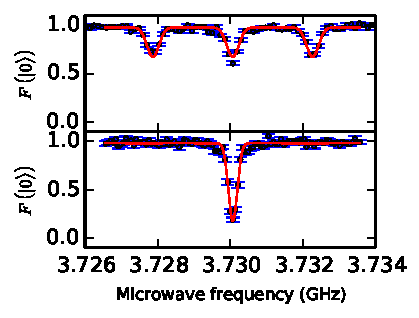
\includegraphics{Img/DarkESR_2.pdf}};
            \node (A) at (2.6,4.4) {};
            \node (B) at (3.92,4.4) { };
            \node (C) at (5.3,4.4) { };
            \draw[latex-latex, font=\small] (A) -- node[label =270: $A_\mathrm{N}$] {} (B);
            \draw[latex-latex, font=\small] (B) -- node[label =270: $A_\mathrm{N}$] {} (C);
        \end{tikzpicture}
        \caption{ Electron Spin Resonance (ESR) for uninitialized (top) and initialized nitrogen spin (bottom) of the $m_s =0 \rightarrow m_s = +1$ transition. In a dark ESR the spin is prepared in $\ket{0}$, a microwave pulse is applied and then the $\ket{0}$ state is read-out again. This is done for a range of frequencies. When the microwave is on resonance with a transition the spin will be rotated and a dip will be visible in the signal. In the top figure the transition is split due to the interaction with the nearby nitrogen atom. In the lower figure the nitrogen state is initialized and the splitting disappears.}
        \label{fig:HF_split_levels}
    \end{figure}

Because the interaction is spin-dependent it can be used to measure the nitrogen's spin state.
Every time an experiment is started the nitrogen starts out in a mixed state.
This means that every time an uninitialized nitrogen is measured it is equally likely to end up in one of its three states.
The nitrogen state can be measured by initializing the electron in the split $m_s = +1$ state and driving one of the transitions to $m_s=0$.
Only if the nitrogen was in the state corresponding to the transition being driven will a measurement of the $m_s =0$ state give a positive result.

By resetting and repeating this procedure until a positive result is measured the nitrogen-spin can be initialized.
The system can be reset into a mixed state by applying a high-energy off-resonant laser pulse.
This procedure is known as Measurement Based Initialization (MBI) and is used in our experiments.
The lower panel of \cref{fig:HF_split_levels} shows an ESR after the nitrogen has been initialized using MBI.

\subsection{Strongly coupled spins}
The ability to control spin states relies on being able to selectively address its spin dependent transitions.
When two transitions can be resolved in an ESR they can be addressed by applying microwave pulses of the corresponding frequencies.
However if two transitions overlap in an ESR, applying a microwave pulse at the corresponding frequency will address both transitions and it is not possible to control its spin state.

Two transitions cannot be resolved when the splitting between them is smaller than the width of the transition.
The magnitude of the splitting is determined by the strength of the interaction and the broadening of the transitions is caused by decoherence.
We define a spin to be strongly coupled when it is possible to readily resolve it's transitions in an ESR experiment with negligible power broadening.
Conversely a spin is weakly coupled when it is not possible to readily resolve its transitions in an ESR.

Strongly coupled spins can be controlled by applying microwaves directly at the transition frequency, weakly coupled spins can not.
Using this method strongly-coupled carbon-13 spins have been controlled and initialized\citep{Robledo2011HighFidelity}.

\section{Decoherence}
The ESR signal is broadened because the NV-center interacts with an environment known as the spin bath.
The spin bath consists of a very large number of spins that are all very weakly coupled to the NV-center.
Just like the uninitialized nitrogen spin these are in a mixed state.
This means that for every iteration of an experiment the spin bath can have a different configuration.
These different configurations of the spin bath slightly shift the addressed transition around causing the broadening of the transition.

\subsection{Decoherence time}
These variations in the spin-bath configuration can be measured with a Ramsey experiment.
In a Ramsey experiment (\cref{fig:Ramsey_gijs}) the electronic spin is brought into a superposition between the $\ket{0}$ and $\ket{1}$-state where it freely evolves for a time $\tau$.
A final pulse brings the state back into $\ket{0}$ where it is read out.

By applying a slight detuning to the rotating frame used to keep the phase fixed an oscillation can be seen in the signal (\cref{fig:electron_T2*}).
Due to the different spin-bath configurations the evolution frequency varies slightly between experiments, this causes the measured signal to decay as the different oscillations move out of phase with each other.
The decay is known as decoherence and the $1/e$-time of the decay is known as the decoherence time.

For a Ramsey experiment the decay follows a Gaussian profile \cref{eq:Ramsey_decay}.
$T_2^*$ is defined as the $1/e$ time of the decay as measured by a Ramsey experiment.
The $T_2^*$ of our sample was measured to be $T_{2,e}^* = 4.54 \pm 14 \mu\mathrm{s}$ with initialized nitrogen-spin.
The decay follows a Gaussian profile within two $\sigma$: $n = 1.81 \pm 0.14$

\begin{equation}
    K(\tau) = e^{-(\tfrac{\tau}{T_{2e}^*})^2}
    \label{eq:Ramsey_decay}
\end{equation}

\begin{figure}[htbp]
    \centering
    \begin{subfigure}[t]{0.49\textwidth}\centering
        \caption{}
        \includegraphics{Img/Ramsey_Gijs.pdf}
        \label{fig:Ramsey_gijs}
    \end{subfigure}
    \begin{subfigure}[t]{0.49\textwidth}\centering
        \caption{}
        \includegraphics{Img/electron_T2star.pdf}
        \label{fig:electron_T2*}
    \end{subfigure}
        \caption{
        \Cref{fig:Ramsey_gijs}, schematic representation of a Ramsey experiment. Figure from \citet{Lange2012Quantum}.
        In a Ramsey experiment a qubit is brought into the $xy$-plane by a $\pi/2$-pulse where it evolves freely for a time $\tau$ before being subjected to a final $\pi/2$ pulse to read out its $x$-component.
        By applying a detuning to the rotating frame the spin will pick up a phase $\phi = \omega_d \tau$ during free evolution.
        The final pulse will rotate the spin towards the poles depending on the phase picked up during free evolution.
        This manifests itself as an oscillation.
        Because the configuration of the spin-bath is slightly different between experiments the frequency of the oscillation will vary with each iteration.
        This variation in frequency between iterations will cause the oscillation to decay.
        \Cref{fig:electron_T2*} shows a Ramsey experiment for the electronic spin.
        A $T_{2,e}^*$ of $4.54 \pm 0.14 \mu\mathrm{s}$ was measured for the electronic spin. The decay follows a Gaussian profile within uncertainty $n = 1.81 \pm 0.14$. }
\end{figure}


\subsection{Relation between decoherence and transition broadening}
The decay in a Ramsey experiment is a measure for variations of the spin-bath in the time-domain while the broadening of transitions in an ESR is a measure for variations of the spin-bath in the frequency domain.
The decay of the Ramsey and the shape of the ESR are related trough a Fourier transform and described by \cref{eq:ESR_dip_shape} \footnote{Assuming negligible power broadening in the ESR, and linear response (How do i explain clearly that in low power regime, not driving all the way trough?)}.
Where $C$ is a constant that depends on the duration and power of the ESR microwave pulse.
Because the decay of the Ramsey is Gaussian the shape of a transition in the ESR is also Gaussian.

\begin{equation}
    \mathcal{F} \{ K(\tau) \} =  C e^{-\tfrac{(2\pi \cdot f) ^2 \cdot T_{2e}^{*2}}{ 4}}
    \label{eq:ESR_dip_shape}
\end{equation}

Two identical Gaussians can be readily resolved when the separation between their maxima is larger than their full-width-half-maximum (FWHM).
The FWHM (in Hz) of the ESR is given by \cref{eq:FWHM}.
\begin{equation}
    \mathrm{FWHM} =  \frac{2\sqrt{\ln{2}}}{\pi T_{2e}^*}
    \label{eq:FWHM}
\end{equation}

An estimation of when carbon spins can be resolved can be made by looking at the strength of the hyperfine interaction.
The splitting caused by a carbon spin is equal to twice the total interaction strength $A$ at low magnetic field ($\gamma_e B \ll A$).
At high field ($\gamma_e B \gg A$) the secular approximation is valid and the splitting is twice the parallel component of the hyperfine $A_\parallel$.
We can readily resolve a transition when the shift due to the corresponding interaction is larger than the FWHM of the transition.

At a natural concentration of carbon-13 NV-centers have a typical  electron $T_{2e}^* \approx 2\mu \mathrm{s}$ that depends on the exact configuration of the spin-environment.
Increasing the carbon-13 concentration generally reduces $T_{2e}^*$.
On the sample used for the experiments $T_{2e}^*=4.54 \pm 0.14 \mu\mathrm{s}$ was measured.
This means that the hyperfine coupling must be larger than $2\pi\cdot$265kHz in a typical NV-center, and larger than $2\pi\cdot$ 117kHz in the sample used in this thesis for a carbon to be strongly coupled.

As the presence of strongly coupled carbons close to the NV-center is governed by probability and the probability of getting 3-5 strongly coupled carbons is very low it is necessary to develop methods to address weakly coupled carbons.
The next chapter will demonstrate methods to extend the coherence time and address weakly coupled carbons, thereby enlarging the spin-register.

